% TikZ figure for the sampling pipeline
% Requires: \usepackage{tikz}
%           \usetikzlibrary{arrows,positioning,fit,calc,shapes.geometric}

\begin{tikzpicture}[
    >=stealth,
    node distance=0.4cm,
    stage/.style={
        draw,
        rounded corners=8pt,
        minimum height=2.8cm,
        minimum width=2.4cm,
        align=center,
        font=\small
    },
    arrow/.style={
        ->,
        thick,
        draw=gray!70,
        line width=2pt,
        shorten >=2pt,
        shorten <=2pt
    },
    bigarrow/.style={
        draw=gray!50,
        line width=2pt,
        shorten >=2pt,
        shorten <=2pt,
        -{Stealth[length=8pt,width=8pt]}
    },
    vec/.style={
        font=\scriptsize,
        inner sep=1pt
    },
    veclabel/.style={
        font=\small\itshape,
        above=2pt
    },
    treenode/.style={
        circle,
        draw,
        minimum size=14pt,
        inner sep=0pt,
        font=\scriptsize
    },
    treeedge/.style={
        draw,
        thick
    }
]

% Stage 1: Sample correlated firings
\node[stage] (stage1) {
    \raisebox{-.5\height}{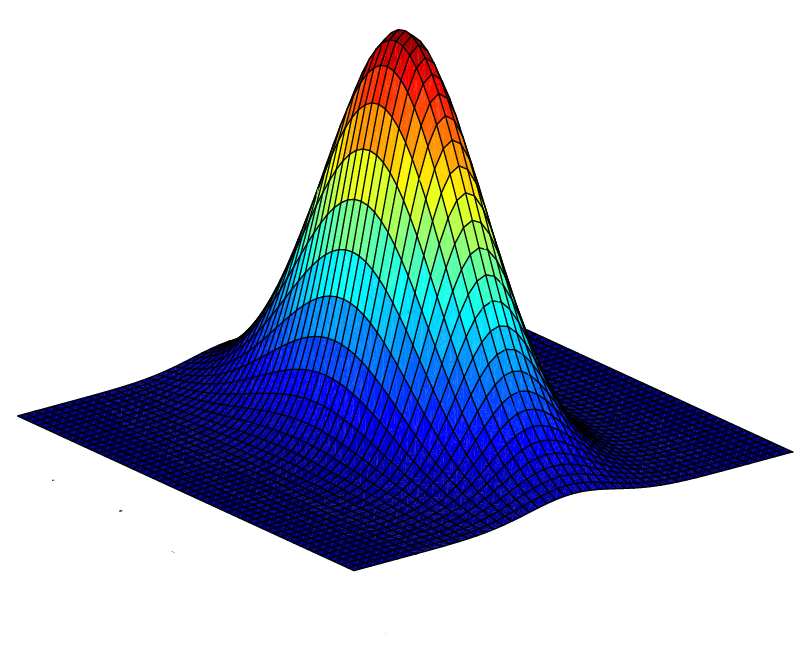
\includegraphics[width=1.4cm]{assets/gaussian.png}}%
    \hspace{4pt}$> \tau$
};
\node[above=0.1cm of stage1, font=\small] {Sample correlated firings};

% Vector z
\node[right=0.6cm of stage1] (z) {
    \scriptsize
    \setlength{\tabcolsep}{2pt}
    \begin{tabular}{|c|}
    \hline
    \rule[-1pt]{0pt}{8pt}\makebox[2em][c]{1} \\ \hline
    \rule[-1pt]{0pt}{8pt}\makebox[2em][c]{1} \\ \hline
    \rule[-1pt]{0pt}{8pt}\makebox[2em][c]{0} \\ \hline
    \rule[-1pt]{0pt}{8pt}\makebox[2em][c]{0} \\ \hline
    \rule[-1pt]{0pt}{8pt}\makebox[2em][c]{0} \\ \hline
    \rule[-1pt]{0pt}{8pt}\makebox[2em][c]{0} \\ \hline
    \rule[-1pt]{0pt}{8pt}\makebox[2em][c]{1} \\ \hline
    \end{tabular}
};
\node[veclabel] at (z.north) {$z$};

% Arrow 1
\draw[bigarrow] (stage1.east) -- (z.west);

% Stage 2: Sample magnitudes
\node[stage, right=0.6cm of z] (stage2) {
    $z \odot \mathcal{N}(\mu, \sigma)$
};
\node[above=0.1cm of stage2, font=\small] {Sample magnitudes};

% Arrow 2
\draw[bigarrow] (z.east) -- (stage2.west);

% Vector c1
\node[right=0.6cm of stage2] (c1) {
    \scriptsize
    \setlength{\tabcolsep}{2pt}
    \begin{tabular}{|c|}
    \hline
    \rule[-1pt]{0pt}{8pt}\makebox[2em][c]{1.3} \\ \hline
    \rule[-1pt]{0pt}{8pt}\makebox[2em][c]{0.9} \\ \hline
    \rule[-1pt]{0pt}{8pt}\makebox[2em][c]{0} \\ \hline
    \rule[-1pt]{0pt}{8pt}\makebox[2em][c]{0} \\ \hline
    \rule[-1pt]{0pt}{8pt}\makebox[2em][c]{0} \\ \hline
    \rule[-1pt]{0pt}{8pt}\makebox[2em][c]{0} \\ \hline
    \rule[-1pt]{0pt}{8pt}\makebox[2em][c]{3.2} \\ \hline
    \end{tabular}
};
\node[veclabel] at (c1.north) {$c$};

% Arrow 3
\draw[bigarrow] (stage2.east) -- (c1.west);

% Stage 3: Enforce hierarchy
\node[stage, right=0.6cm of c1, minimum width=3.2cm] (stage3) {
    \begin{tikzpicture}[scale=1.0]
        % Tree structure - increased spacing
        \node[treenode] (n1) at (0,0) {1};
        \node[treenode] (n2) at (-0.7,-0.7) {2};
        \node[treenode] (n3) at (0.7,-0.7) {3};
        \node[treenode] (n4) at (-1.05,-1.4) {4};
        \node[treenode] (n5) at (-0.35,-1.4) {5};
        \node[treenode] (n6) at (0.35,-1.4) {6};
        \node[treenode] (n7) at (1.05,-1.4) {7};
        \draw[treeedge] (n1) -- (n2);
        \draw[treeedge] (n1) -- (n3);
        \draw[treeedge] (n2) -- (n4);
        \draw[treeedge] (n2) -- (n5);
        \draw[treeedge] (n3) -- (n6);
        \draw[treeedge] (n3) -- (n7);
    \end{tikzpicture}
};
\node[above=0.1cm of stage3, font=\small] {Enforce hierarchy};

% Arrow 4
\draw[bigarrow] (c1.east) -- (stage3.west);

% Vector c2
\node[right=0.6cm of stage3] (c2) {
    \scriptsize
    \setlength{\tabcolsep}{2pt}
    \begin{tabular}{|c|}
    \hline
    \rule[-1pt]{0pt}{8pt}\makebox[2em][c]{1.3} \\ \hline
    \rule[-1pt]{0pt}{8pt}\makebox[2em][c]{0.9} \\ \hline
    \rule[-1pt]{0pt}{8pt}\makebox[2em][c]{0} \\ \hline
    \rule[-1pt]{0pt}{8pt}\makebox[2em][c]{0} \\ \hline
    \rule[-1pt]{0pt}{8pt}\makebox[2em][c]{0} \\ \hline
    \rule[-1pt]{0pt}{8pt}\makebox[2em][c]{0} \\ \hline
    \rule[-1pt]{0pt}{8pt}\makebox[2em][c]{0} \\ \hline
    \end{tabular}
};
\node[veclabel] at (c2.north) {$c$};

% Arrow 5
\draw[bigarrow] (stage3.east) -- (c2.west);

% Stage 4: Apply feature dictionary
\node[stage, right=0.6cm of c2] (stage4) {
    $\mathbf{D}^\top c + \mathbf{b}$
};
\node[above=0.1cm of stage4, font=\small] {Apply feature dictionary};

% Arrow 6
\draw[bigarrow] (c2.east) -- (stage4.west);

% Vector a
\node[right=0.6cm of stage4] (a) {
    \scriptsize
    \setlength{\tabcolsep}{2pt}
    \begin{tabular}{|c|}
    \hline
    \rule[-1pt]{0pt}{8pt}\makebox[2em][c]{-2.1} \\ \hline
    \rule[-1pt]{0pt}{8pt}\makebox[2em][c]{1.9} \\ \hline
    \rule[-1pt]{0pt}{8pt}\makebox[2em][c]{-0.1} \\ \hline
    \rule[-1pt]{0pt}{8pt}\makebox[2em][c]{0.7} \\ \hline
    \end{tabular}
};
\node[veclabel] at (a.north) {$a$};

% Arrow 7
\draw[bigarrow] (stage4.east) -- (a.west);

\end{tikzpicture}
